\begin{figure}[!htbp]
\centering
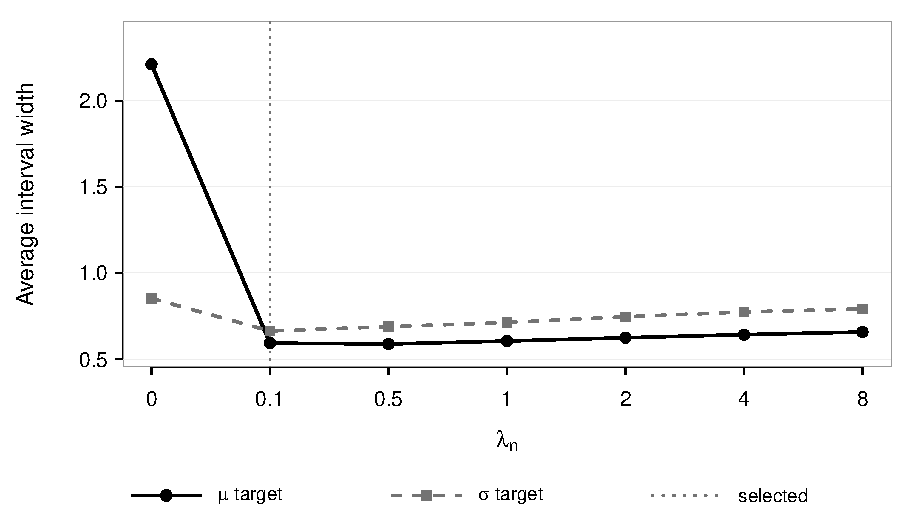
\includegraphics[width=0.76\linewidth]{results/figures/fig_sens_lambda.pdf}
\caption{Sensitivity to the penalty weight $\lambda_n$: average interval width for each target. Grid points are drawn at equal ordinal spacing because the design grid is geometric; the dotted line marks the selected value $\lambda_n=0.1$. The $\mu$-target width falls from $2.213$ at $\lambda_n=0$ to $0.593$ at the selected value and then rises slowly. Coverage clears the Monte-Carlo-adjusted floor at every grid point, so the figure concerns width alone.}
\label{fig:sens-lambda}
\end{figure}
